



% \section{Deep Learning - Microsoft}

% 	\subsection{Name of networks}
% 		deep belief network (DBN), 
% 		deep neural networks (DNN), recurentneural networks (RNN), convolutional neural networks (CNN).
% 		restricted Boltzmann machine (DBM), regularized autoencoders
% 		TABLE 3.1 !!

% 	\subsection{Unsupervised vs supervised}
% 		"deep supervised learnings are usually more efficient to train and test, more flexible to construct, and more suitable for end-to-end learning of complex systems."

% 		"The deep-unsupervised models are easier to interpret, easier to embed domain knowledge, easier to compose, and easier to handle uncertainty, but they are typically intractable in inference and learning for complex systems"


% 	\subsection{Unsupervised, supervised, hybrid}
% 		Deep learning is decomposed on three major classes: the deep network for unsupervised learning, the deep network for supervised learning and the deep network for hybrid learning.

% 		The deep network for unsupervised learning intend to capture patterns in the input data when no informations are given about the output. They are referred as "unsupervised feature learning" or "representation learning"

% 		The deep network for supervised learning are intended to discriminate the inputs. In contradiction with the unsupervised learning, the patterns recognized are often characterized by the output of the data.

% 		The hybrid deep networks ... will see


% 	\subsubsection{Unsupervised networks}
% 		The unsupervised learning networks are often based on energy functions.



% \section{Deep Learning - MIT}
	
% 	\subsection{Introduction}
% 		The idea behind creating a deep learning model comes from the brain. Back in 1959, Hubel and Wiesel \ref{article:visual_cortex} studied the visual cortex of cats. They discovered that neurons triggered when recognizing edges and that visual information were processed through many layers on the brain. Based on those observations 



\section{Deep Learning - Bengio}
\label{sec:deep_learning}	

	\subsection{Gradient Descent}
		Most of deep learning algorithms are about optimizing a cost function $f(x|\theta)$ where $x$ is the input and $\theta$ are some parameters. This cost function can have multiple input but has to have one output $f:\mathbb{R}^n\rightarrow \mathbb{R}$. Optimizing this function is retrieving it's global minimum (or maximum), in other words, finding what are the parameters $\theta$ so that the function is minimum. 

		A famous method is based on derivatives. Consider a function $f:\mathbb{R}^2 \rightarrow \mathbb{R}$. We can find its minimum searching for the zeros of its derivative. A derivative equal to zero at $x_1$ can mean that $f(x_1)$ is either a local minimum, a global minimum, a plateau, a local maximum or a global maximum. As we notice, finding a derivative equal to zero is not enough.

		In the general case of deep learning we have multidimensional inputs which makes derivatives inapplicable. The method we use is called Gradient Descent. It is bases itself on the idea described above. Instead of derivative, it uses the gradient of the cost function $\nabla_x f(x)$. The gradient is a vector containing all the partial derivatives $\frac{\partial}{\partial_{x_i}}f(x)$. We can't evaluate the derivative of the entire function given the inputs therefore we use an iterative process to find the minimum. Conceptually, we begin at a point $x_1$ and compute the gradient at this point. From this gradient you get insight on what direction to take to minimize the function so you take a step towards that direction. You update your position by $x_{update} = x - \epsilon \nabla_x f(x)$ where $\epsilon$ is a step size.


	\subsection{Back-Propagation}
		In deep learning, back-propagation is the method we use to compute the gradient of the cost-function.

		back-propagation algorithm take adventage of the chain rule:
		\begin{equation}
			\frac{\partial C(h(x))}{\partial x} = \frac{\partial C(h(x))}{\partial h(x)} \frac{\partial h(x)}{\partial x}
		\end{equation}
		Where $C(f)$ is the cost function, $h(x)$ is a hidden layer and $x$ is an input to the graph. As we can notice, the initial problem is to know what is the partial derivative of the cost-function given the input $x$. Thanks to the chain rule, we can propagate the derivative through the layers of the network. \Fref{fig:back_prop1} shows a simple, three nodes, directed graph. It has the functions mention above and we see how a change in $z$ is influanced by a change in $x$. In the case of multiple varaibles ingoing the cost function (when you have many hidden neurons on a layer for instance), the chain rule is written as follow:
		\begin{equation}
			\frac{\partial C(h(x))}{\partial x} = \sum_i\frac{\partial C(h_i(x))}{\partial h(x)} \frac{\partial h_i(x)}{\partial x}
		\end{equation}
		where $h(x)$ is a vector.


		\usetikzlibrary{calc,trees,positioning,arrows,chains,shapes.geometric,%
		decorations.pathreplacing,decorations.pathmorphing,shapes,%
		matrix,shapes.symbols}

		\tikzset{
		>=stealth',
			node/.style={circle, draw=black, very thick,
				text width=1em, text centered, on chain},
			nod2/.style={circle, draw=black, very thick,
				text width=3em, text centered},
			every join/.style={<-, thick,shorten >=1pt},
			annot/.style={text width=6em, text centered},
		}

		\begin{figure}
			\centering
			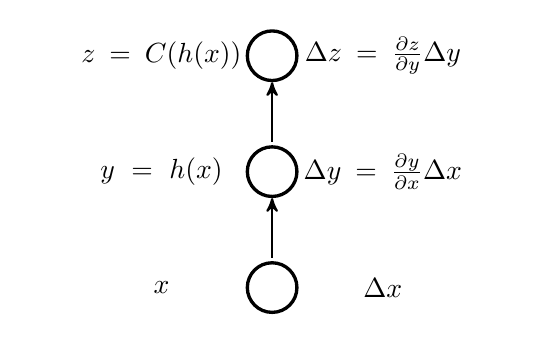
\begin{tikzpicture} 
				[node distance=.8cm,
				start chain=going below,]
				\node[node, join] (cost)   {};
				\node[node, join] (hidden) {};
				\node[node, join] (input)  {};

				\node[annot,left of=cost  , node distance=4em] (a) {$z = C(h(x))$};
				\node[annot,left of=hidden, node distance=4em] (b) {$y = h(x)$};
				\node[annot,left of=input , node distance=4em] (c) {$x$};

				\node[annot,right of=cost  , node distance=4em] (a) {$ \Delta z = \frac{\partial z}{\partial y} \Delta y$};
				\node[annot,right of=hidden, node distance=4em] (b) {$ \Delta y = \frac{\partial y}{\partial x} \Delta x$};
				\node[annot,right of=input , node distance=4em] (c) {$ \Delta x$};

			\end{tikzpicture}
			\caption{simple directed graph}
			\label{fig:back_prop1}
		\end{figure}


	Now that we saw how the back propagation was applied in a simple chain of nodes, we will see how does it do in a more general case of deep neural network fully connected. Now, the cost-function takes multiple parameters, there is many hidden layers and an input layer of many variables. \Fref{fig:back_prop2} shows an illustration of this generic network where $u_i = f_i(u_j)$ with $j \in parents(i)$.


	The algorithm works as follow:
	We want to figure out if the parameter (weights) we have learned so far are correct (which they must likely aren't). If they are incorrect we want to modify them so they diminish the error of our network. We consider the network represented on \fref{fig:back_prop2}. As always, we have an input vector $x$ and an output (prediction) layer $t$. We then have some hidden layers. $x_j^{(n)}$ where $n \in [0,N]$ is the layer number and $j$ is the index of the neuron in the layer. We also denote $w_{ji}$ the weight from neuron $x_i^{(n-1)}$ to neuron $x_j^{(n)}$.
	In this network, a neuron has a activation function $g$ and a aggregation function $h$. As in the general case we'll consider in this example the function $h$ to be the sum of the product of both the weight and the input of the neuron: $h = \sum_i w_{ji}^n w_i^{[n-1)}$

		\begin{figure}
		\centering
		\def\layersep{3em}

		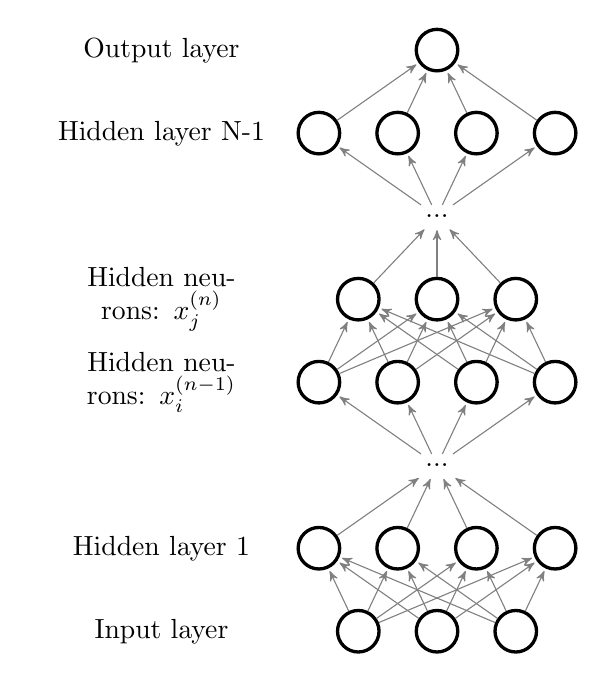
\begin{tikzpicture}[shorten >=1pt,->,draw=black!50, node distance=\layersep]
			\tikzstyle{every pin edge}=[<-, thick,shorten >=1pt]
			\tikzstyle{neuron}=[circle,draw=black, very thick,,minimum size=1.5em,inner sep=0em]
			\tikzstyle{annot} = [text width=9em, text centered]
			\tikzstyle{annot2} = [text width=6em, text centered]

			
			% --------------
			%   Draw nodes
			% --------------
			\node[neuron] (O) at (2.5,\layersep*7) {}; % Draw output node
			
			\foreach \name / \y in {1,...,4} % Draw the hidden4 nodes
				\node[neuron] (H4-\name) at (\y+0.0,\layersep*6) {};

				\node[annot]  (N2-1)     at (2.5   ,\layersep*5)  {...};

			\foreach \name / \y in {1,...,3} % Draw the hidden3 nodes
				\node[neuron] (H3-\name) at (\y+0.5,\layersep*4) {};

			\foreach \name / \y in {1,...,4} % Draw the hidden2 nodes
				\node[neuron] (H2-\name) at (\y+0.0,\layersep*3) {};

				\node[annot]  (N1-1)     at (2.5   ,\layersep*2)  {...};

			\foreach \name / \y in {1,...,4} % Draw the hidden1 nodes
				\node[neuron] (H1-\name) at (\y+0.0,\layersep*1) {};

			\foreach \name / \y in {1,...,3} % Draw the input nodes
				\node[neuron] (I-\name) at  (\y+0.5,\layersep*0) {};


			% -----------------
			%   Connect nodes
			% -----------------
			\foreach \source in {1,...,4} % connect hidden4 & out
				\path (H4-\source) edge (O);

			\foreach \source in {1,...,1} % connect Null2 & hidden4
				\foreach \dest in {1,...,4}
					\path (N2-\source) edge (H4-\dest);

			\foreach \source in {1,...,3} % connect hidden3 & Null2
				\foreach \dest in {1,...,1}
					\path (H3-\source) edge (N2-\dest);

			\foreach \source in {1,...,4} % connect hidden2 & hidden3
				\foreach \dest in {1,...,3}
					\path (H2-\source) edge (H3-\dest);

			\foreach \source in {1,...,1} % connect Null1 & hidden2
				\foreach \dest in {1,...,4}
					\path (N1-\source) edge (H2-\dest);	

			\foreach \source in {1,...,4} % connect hidden1 & Null1
				\foreach \dest in {1,...,1}
					\path (H1-\source) edge (N1-\dest);

			\foreach \source in {1,...,3} % connect input & hidden1
				\foreach \dest in {1,...,4}
					\path (I-\source) edge (H1-\dest);	


			% Annotate the layers
			\node[annot] at (-1,\layersep*7) {Output layer};
			\node[annot] at (-1,\layersep*6) {Hidden layer N-1};
			\node[annot] at (-1,\layersep*4) {Hidden neurons: $x_j^{(n)}$  };
			\node[annot] at (-1,\layersep*3) {Hidden neurons: $x_i^{(n-1)}$};
			\node[annot] at (-1,\layersep*1) {Hidden layer 1};
			\node[annot] at (-1,\layersep*0) {Input layer};
			% \node[annot2] () at (5,\layersep*4) {$u_i = f_i(u_j)$};
			% \node[annot2] () at (5,\layersep*3) {$u_j$};

		\end{tikzpicture}

		\caption{fully connected N layer neural network}
		\label{fig:back_prop2}
	\end{figure}

	The first step of the algorithm is to compute the error of our network. We do it using forward propagation. The idea is to compute the cost function going through all neurons beginning from the input layer up to the output layer. So we should update the neurons following the next formula:

	\begin{equation}
		x_j^{(n)} = g^{(n)}(h_j^{(n)})
	\end{equation}

	We begin at $n=1$ and go iteratively up to $n=N$. Therefore, the $n^{th}$ result can take the advantage of the $(n-1)^{th}$ result computed on a preceding step.

	
	Then we back-propagate the error in order to get the gradient of the error function in terms of its weights. We do this using the chain rule seen above.

	\begin{algorithm}[H]
		\KwResult{returns a set of partial derivatives for every hidden nodes}
		\BlankLine
		\emph{\% Compute error on output layer}\;
		\For{$i \leftarrow 1$ \KwTo $I$}{
			$e^{out} \leftarrow g'^{(out)}(h_i^{(out)})[t_i-y_i]$\;
		}
		\emph{\% back propagate error throughout the network}\;
		\For{$n \leftarrow 1$ \KwTo $N$}{
			\For{$j \leftarrow 1$ \KwTo $J$}{
				$e_j^{(n-1)} \leftarrow g'^{(n-1)}(h_j^{(n-1)})h'^{(n-1)}$\;
			}
		}
		\Return $(e_i^n)_{n\in[1,N], i\in[1,size(e^n)]}$
	\caption{Back propagation}
	\label{alg:back_propagation}
	\end{algorithm}
	
	We can notice here that in the general case we assumed above (for $h = \sum_i w_{ji}^n w_i^{[n-1)}$), the update formula become: 
	\begin{equation}
		e_j^{(n-1)} \leftarrow g'^{(n-1)}(h_j^{(n-1)}) \sum_{i\in parent(j)} w_{ji} e_i^{n}
	\end{equation}
	The last step of the algorithm is to update the weights of the vector so that its error can diminish. The update formula is: $\Delta w_{ij}^n = \lambda e_i^{(n)} x_j^{(n-1)}$ where $\lambda$ is the learning rate.



	\subsection{Linear regression}
		The first machine intelligence algorithm we will talk about is the linear regression. Here the task $T$ is regression. Regression  is about learning a function that maps the input $x$ to a real value. It is defined as $f:\mathbb{R}^n \rightarrow \mathbb{R}$. In a two dimension space, regression learns a curve going through labeled data.
		Linear regression is about learning  a linear function of the input. We define the prediction $\hat{y}$ as: $\hat{y}=W^Tx$ where $x$ is the input data, $W$ is a weight vector. Here, each input feature $x_i$ is multiplied by a coefficient $w_i$ then summed up to get the prediction. The vector $W$ weights each input feature giving more or less importance to one or the other feature.\\


		Once the task is defined, we chose a performance measure $P$. This measure reflects the accuracy of the model. We evaluate the data on a test set different from the training set. 
		In the example of linear regression one can use the mean squared error. We consider $y^{test}$ the valid output for the test set and $\hat{y}^{test}$ our prediction for the test set. The mean squared error is given by
		\begin{equation}
			\begin{split}
				MSE_{test} &= \frac{1}{m}\sum_{i}(\hat{y}^{test}	- y^{test})_i^2 \\
				MSE_{test} &= \frac{1}{m}   \norm{\hat{y}^{test}	- y^{test}}_2^2
			\end{split}
		\end{equation}

		When $y^{test}$ is close to $\hat{y}^{test}$ the mean square error is low. This is exactly what we want. Modify the weights $W$ so that they minimizes $MSE_{train}$. We search for local minimum thanks to gradients

		\begin{equation} \label{eq1}
			\begin{split}
				\nabla_W MSE &= 0 \\
				\nabla_W \frac{1}{m} \norm{\hat{y} - y}_2^2 &= 0 \\
				\frac{1}{m} \nabla_W \norm{\hat{y} - y}_2^2 &= 0 \\
				\nabla_W (\hat{y} - y)(\hat{y} - y) &= 0 \\
				\nabla_W (X w - y)(X w - y) &= 0 \\
				\nabla_W (w^T X^T X w - 2 w^T X^T y + y^T y) &= 0 \\
				\nabla_W (2 X^T X w - 2 X^T y) &= 0 \\
				(X^T X)^{-1} X^T y &= w
			\end{split}
		\end{equation}

		In order to find the local minimum, one can just compute the last line of the equation and retrieve the optimal value for w on the given set.


	\subsection{Multi Layer Perceptron}


